\documentclass{standalone}
\usepackage{tikz}
\usetikzlibrary{patterns, positioning}


\begin{document}
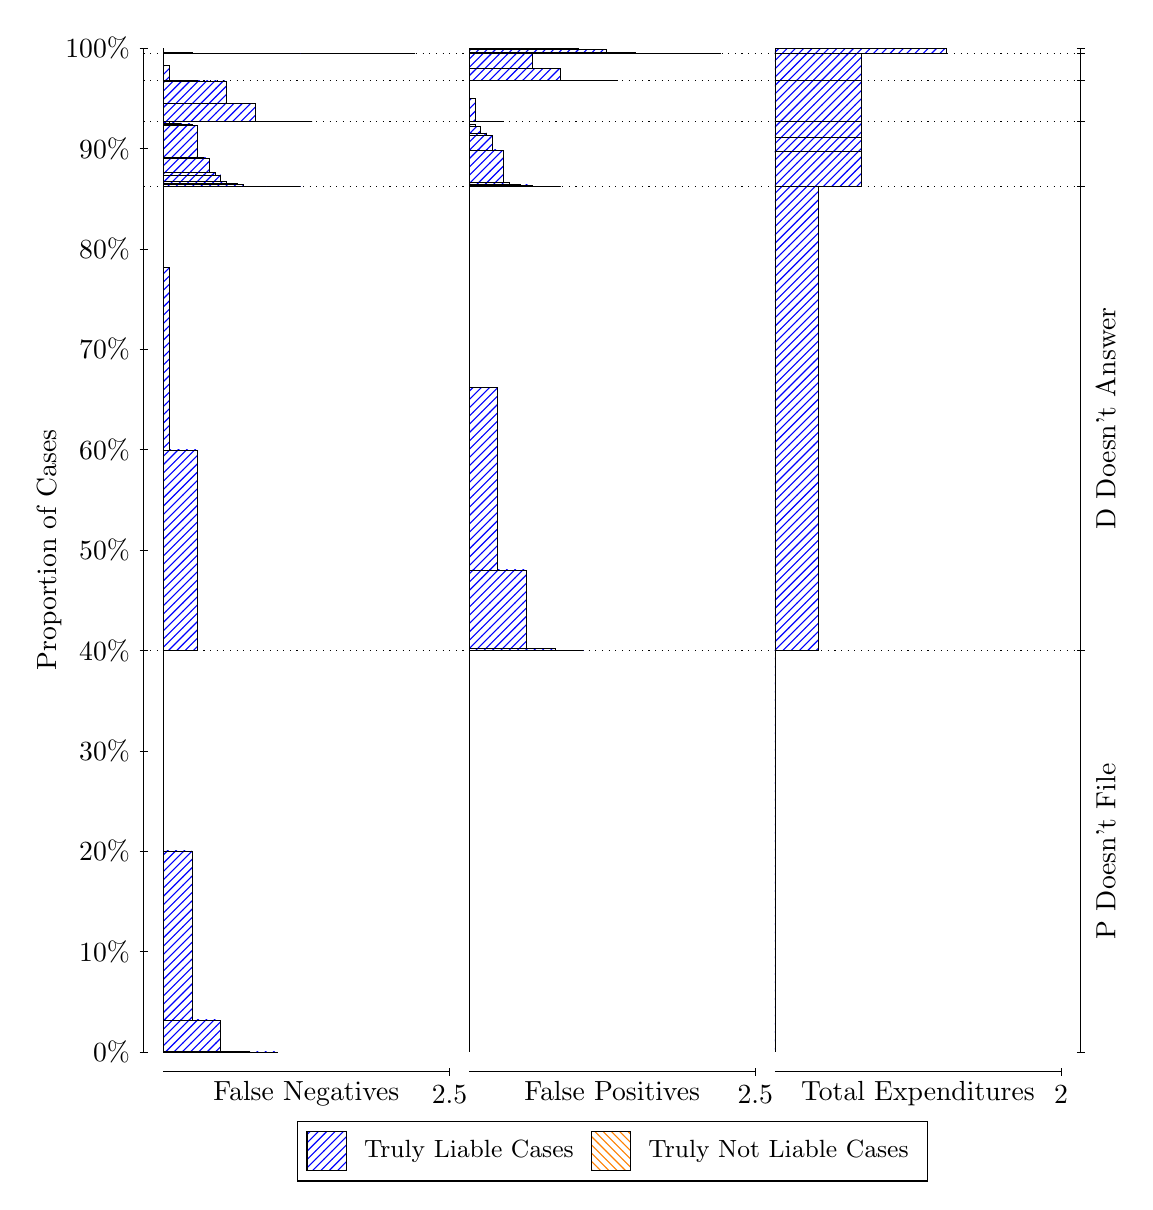
\begin{tikzpicture}
\draw[black, very thin] (1.5,1.75) -- (1.5,14.5);
\node[rotate=90, text=black, anchor=center] at (0.3, 8.125) {Proportion of Cases};
\draw[black, very thin] (1.45,1.75) -- (1.55,1.75);
\node[text=black, anchor=east] at (1.45, 1.75) {0\%};
\draw[black, very thin] (1.45,3.025) -- (1.55,3.025);
\node[text=black, anchor=east] at (1.45, 3.025) {10\%};
\draw[black, very thin] (1.45,4.3) -- (1.55,4.3);
\node[text=black, anchor=east] at (1.45, 4.3) {20\%};
\draw[black, very thin] (1.45,5.575) -- (1.55,5.575);
\node[text=black, anchor=east] at (1.45, 5.575) {30\%};
\draw[black, very thin] (1.45,6.85) -- (1.55,6.85);
\node[text=black, anchor=east] at (1.45, 6.85) {40\%};
\draw[black, very thin] (1.45,8.125) -- (1.55,8.125);
\node[text=black, anchor=east] at (1.45, 8.125) {50\%};
\draw[black, very thin] (1.45,9.4) -- (1.55,9.4);
\node[text=black, anchor=east] at (1.45, 9.4) {60\%};
\draw[black, very thin] (1.45,10.675) -- (1.55,10.675);
\node[text=black, anchor=east] at (1.45, 10.675) {70\%};
\draw[black, very thin] (1.45,11.95) -- (1.55,11.95);
\node[text=black, anchor=east] at (1.45, 11.95) {80\%};
\draw[black, very thin] (1.45,13.225) -- (1.55,13.225);
\node[text=black, anchor=east] at (1.45, 13.225) {90\%};
\draw[black, very thin] (1.45,14.5) -- (1.55,14.5);
\node[text=black, anchor=east] at (1.45, 14.5) {100\%};

\draw[black, very thin] (13.4,1.75) -- (13.4,14.5);
\draw[black, very thin] (13.35,1.75) -- (13.45,1.75);
\node[anchor=west] at (13.35, 1.75) {};
\draw[black, very thin] (13.35,6.8489) -- (13.45,6.8489);
\node[anchor=west] at (13.35, 6.8489) {};
\draw[black, very thin] (13.35,12.741) -- (13.45,12.741);
\node[anchor=west] at (13.35, 12.741) {};
\draw[black, very thin] (13.35,13.569) -- (13.45,13.569);
\node[anchor=west] at (13.35, 13.569) {};
\draw[black, very thin] (13.35,14.088) -- (13.45,14.088);
\node[anchor=west] at (13.35, 14.088) {};
\draw[black, very thin] (13.35,14.43) -- (13.45,14.43);
\node[anchor=west] at (13.35, 14.43) {};
\draw[black, very thin] (13.35,14.5) -- (13.45,14.5);
\node[anchor=west] at (13.35, 14.5) {};

\draw[black, very thin, pattern color=blue, pattern=north east lines] (1.75,1.75) rectangle (3.2033,1.75);
\draw[black, very thin, pattern color=blue, pattern=north east lines] (1.75,1.75) rectangle (2.84,1.7534);
\draw[black, very thin, pattern color=blue, pattern=north east lines] (1.75,1.7534) rectangle (2.4767,2.158);
\draw[black, very thin, pattern color=blue, pattern=north east lines] (1.75,2.158) rectangle (2.1133,4.3029);
\draw[black, very thin, pattern color=orange, pattern=north west lines] (1.75,4.3029) rectangle (1.75,4.3029);
\draw[black, very thin, pattern color=blue, pattern=north east lines] (1.75,4.3029) rectangle (1.75,6.8489);
\draw[black, very thin, pattern color=blue, pattern=north east lines] (1.75,6.8489) rectangle (2.186,9.3965);
\draw[black, very thin, pattern color=blue, pattern=north east lines] (1.75,9.3965) rectangle (1.8227,11.718);
\draw[black, very thin, pattern color=orange, pattern=north west lines] (1.75,11.718) rectangle (1.75,11.718);
\draw[black, very thin, pattern color=blue, pattern=north east lines] (1.75,11.718) rectangle (1.75,12.741);
\draw[black, very thin, pattern color=blue, pattern=north east lines] (1.75,12.741) rectangle (3.494,12.741);
\draw[black, very thin, pattern color=blue, pattern=north east lines] (1.75,12.741) rectangle (3.3487,12.741);
\draw[black, very thin, pattern color=blue, pattern=north east lines] (1.75,12.741) rectangle (3.2033,12.741);
\draw[black, very thin, pattern color=blue, pattern=north east lines] (1.75,12.741) rectangle (3.1307,12.741);
\draw[black, very thin, pattern color=blue, pattern=north east lines] (1.75,12.741) rectangle (3.058,12.741);
\draw[black, very thin, pattern color=blue, pattern=north east lines] (1.75,12.741) rectangle (2.9853,12.741);
\draw[black, very thin, pattern color=blue, pattern=north east lines] (1.75,12.741) rectangle (2.9127,12.741);
\draw[black, very thin, pattern color=blue, pattern=north east lines] (1.75,12.741) rectangle (2.84,12.745);
\draw[black, very thin, pattern color=blue, pattern=north east lines] (1.75,12.745) rectangle (2.7673,12.767);
\draw[black, very thin, pattern color=blue, pattern=north east lines] (1.75,12.767) rectangle (2.6947,12.777);
\draw[black, very thin, pattern color=blue, pattern=north east lines] (1.75,12.777) rectangle (2.622,12.783);
\draw[black, very thin, pattern color=blue, pattern=north east lines] (1.75,12.783) rectangle (2.5493,12.805);
\draw[black, very thin, pattern color=blue, pattern=north east lines] (1.75,12.805) rectangle (2.4767,12.89);
\draw[black, very thin, pattern color=blue, pattern=north east lines] (1.75,12.89) rectangle (2.404,12.918);
\draw[black, very thin, pattern color=blue, pattern=north east lines] (1.75,12.918) rectangle (2.3313,13.106);
\draw[black, very thin, pattern color=blue, pattern=north east lines] (1.75,13.106) rectangle (2.2587,13.112);
\draw[black, very thin, pattern color=blue, pattern=north east lines] (1.75,13.112) rectangle (2.186,13.515);
\draw[black, very thin, pattern color=blue, pattern=north east lines] (1.75,13.515) rectangle (2.1133,13.537);
\draw[black, very thin, pattern color=blue, pattern=north east lines] (1.75,13.537) rectangle (2.0407,13.538);
\draw[black, very thin, pattern color=blue, pattern=north east lines] (1.75,13.538) rectangle (1.968,13.548);
\draw[black, very thin, pattern color=blue, pattern=north east lines] (1.75,13.548) rectangle (1.8953,13.548);
\draw[black, very thin, pattern color=blue, pattern=north east lines] (1.75,13.548) rectangle (1.8227,13.569);
\draw[black, very thin, pattern color=orange, pattern=north west lines] (1.75,13.569) rectangle (1.75,13.569);
\draw[black, very thin, pattern color=blue, pattern=north east lines] (1.75,13.569) rectangle (1.75,13.569);
\draw[black, very thin, pattern color=blue, pattern=north east lines] (1.75,13.569) rectangle (3.6393,13.569);
\draw[black, very thin, pattern color=blue, pattern=north east lines] (1.75,13.569) rectangle (3.276,13.57);
\draw[black, very thin, pattern color=blue, pattern=north east lines] (1.75,13.57) rectangle (2.9127,13.799);
\draw[black, very thin, pattern color=blue, pattern=north east lines] (1.75,13.799) rectangle (2.5493,14.084);
\draw[black, very thin, pattern color=blue, pattern=north east lines] (1.75,14.084) rectangle (2.186,14.088);
\draw[black, very thin, pattern color=orange, pattern=north west lines] (1.75,14.088) rectangle (1.75,14.088);
\draw[black, very thin, pattern color=blue, pattern=north east lines] (1.75,14.088) rectangle (2.186,14.09);
\draw[black, very thin, pattern color=blue, pattern=north east lines] (1.75,14.09) rectangle (1.8227,14.277);
\draw[black, very thin, pattern color=orange, pattern=north west lines] (1.75,14.277) rectangle (1.75,14.277);
\draw[black, very thin, pattern color=blue, pattern=north east lines] (1.75,14.277) rectangle (1.75,14.43);
\draw[black, very thin, pattern color=blue, pattern=north east lines] (1.75,14.43) rectangle (4.9473,14.43);
\draw[black, very thin, pattern color=blue, pattern=north east lines] (1.75,14.43) rectangle (4.584,14.43);
\draw[black, very thin, pattern color=blue, pattern=north east lines] (1.75,14.43) rectangle (4.2207,14.431);
\draw[black, very thin, pattern color=blue, pattern=north east lines] (1.75,14.431) rectangle (3.8573,14.436);
\draw[black, very thin, pattern color=blue, pattern=north east lines] (1.75,14.436) rectangle (3.494,14.436);
\draw[black, very thin, pattern color=blue, pattern=north east lines] (1.75,14.436) rectangle (3.1307,14.436);
\draw[black, very thin, pattern color=blue, pattern=north east lines] (1.75,14.436) rectangle (2.84,14.436);
\draw[black, very thin, pattern color=blue, pattern=north east lines] (1.75,14.436) rectangle (2.4767,14.436);
\draw[black, very thin, pattern color=blue, pattern=north east lines] (1.75,14.436) rectangle (2.1133,14.448);
\draw[black, very thin, pattern color=orange, pattern=north west lines] (1.75,14.448) rectangle (1.75,14.448);
\draw[black, very thin, pattern color=blue, pattern=north east lines] (1.75,14.448) rectangle (1.75,14.5);
\draw[black, very thin, pattern color=orange, pattern=north west lines] (5.6333,1.75) rectangle (5.6333,1.75);
\draw[black, very thin, pattern color=blue, pattern=north east lines] (5.6333,1.75) rectangle (5.6333,6.8489);
\draw[black, very thin, pattern color=orange, pattern=north west lines] (5.6333,6.8489) rectangle (7.0867,6.8489);
\draw[black, very thin, pattern color=blue, pattern=north east lines] (5.6333,6.8489) rectangle (7.0867,6.8489);
\draw[black, very thin, pattern color=blue, pattern=north east lines] (5.6333,6.8489) rectangle (6.7233,6.8779);
\draw[black, very thin, pattern color=blue, pattern=north east lines] (5.6333,6.8779) rectangle (6.36,7.8726);
\draw[black, very thin, pattern color=blue, pattern=north east lines] (5.6333,7.8726) rectangle (5.9967,10.194);
\draw[black, very thin, pattern color=blue, pattern=north east lines] (5.6333,10.194) rectangle (5.6333,12.741);
\draw[black, very thin, pattern color=orange, pattern=north west lines] (5.6333,12.741) rectangle (6.796,12.741);
\draw[black, very thin, pattern color=blue, pattern=north east lines] (5.6333,12.741) rectangle (6.796,12.741);
\draw[black, very thin, pattern color=orange, pattern=north west lines] (5.6333,12.741) rectangle (6.6507,12.741);
\draw[black, very thin, pattern color=blue, pattern=north east lines] (5.6333,12.741) rectangle (6.6507,12.741);
\draw[black, very thin, pattern color=orange, pattern=north west lines] (5.6333,12.741) rectangle (6.5053,12.741);
\draw[black, very thin, pattern color=blue, pattern=north east lines] (5.6333,12.741) rectangle (6.5053,12.741);
\draw[black, very thin, pattern color=blue, pattern=north east lines] (5.6333,12.741) rectangle (6.4327,12.763);
\draw[black, very thin, pattern color=orange, pattern=north west lines] (5.6333,12.763) rectangle (6.36,12.763);
\draw[black, very thin, pattern color=blue, pattern=north east lines] (5.6333,12.763) rectangle (6.36,12.763);
\draw[black, very thin, pattern color=blue, pattern=north east lines] (5.6333,12.763) rectangle (6.2873,12.773);
\draw[black, very thin, pattern color=orange, pattern=north west lines] (5.6333,12.773) rectangle (6.2147,12.773);
\draw[black, very thin, pattern color=blue, pattern=north east lines] (5.6333,12.773) rectangle (6.2147,12.773);
\draw[black, very thin, pattern color=blue, pattern=north east lines] (5.6333,12.773) rectangle (6.142,12.796);
\draw[black, very thin, pattern color=blue, pattern=north east lines] (5.6333,12.796) rectangle (6.0693,13.199);
\draw[black, very thin, pattern color=blue, pattern=north east lines] (5.6333,13.199) rectangle (5.9967,13.205);
\draw[black, very thin, pattern color=blue, pattern=north east lines] (5.6333,13.205) rectangle (5.924,13.393);
\draw[black, very thin, pattern color=blue, pattern=north east lines] (5.6333,13.393) rectangle (5.8513,13.421);
\draw[black, very thin, pattern color=blue, pattern=north east lines] (5.6333,13.421) rectangle (5.7787,13.506);
\draw[black, very thin, pattern color=blue, pattern=north east lines] (5.6333,13.506) rectangle (5.706,13.528);
\draw[black, very thin, pattern color=blue, pattern=north east lines] (5.6333,13.528) rectangle (5.6333,13.569);
\draw[black, very thin, pattern color=orange, pattern=north west lines] (5.6333,13.569) rectangle (6.0693,13.569);
\draw[black, very thin, pattern color=blue, pattern=north east lines] (5.6333,13.569) rectangle (6.0693,13.573);
\draw[black, very thin, pattern color=blue, pattern=north east lines] (5.6333,13.573) rectangle (5.706,13.858);
\draw[black, very thin, pattern color=blue, pattern=north east lines] (5.6333,13.858) rectangle (5.6333,14.088);
\draw[black, very thin, pattern color=orange, pattern=north west lines] (5.6333,14.088) rectangle (7.5227,14.088);
\draw[black, very thin, pattern color=blue, pattern=north east lines] (5.6333,14.088) rectangle (7.5227,14.088);
\draw[black, very thin, pattern color=blue, pattern=north east lines] (5.6333,14.088) rectangle (7.1593,14.088);
\draw[black, very thin, pattern color=blue, pattern=north east lines] (5.6333,14.088) rectangle (6.796,14.241);
\draw[black, very thin, pattern color=blue, pattern=north east lines] (5.6333,14.241) rectangle (6.4327,14.428);
\draw[black, very thin, pattern color=blue, pattern=north east lines] (5.6333,14.428) rectangle (6.0693,14.43);
\draw[black, very thin, pattern color=orange, pattern=north west lines] (5.6333,14.43) rectangle (8.8307,14.43);
\draw[black, very thin, pattern color=blue, pattern=north east lines] (5.6333,14.43) rectangle (8.8307,14.43);
\draw[black, very thin, pattern color=blue, pattern=north east lines] (5.6333,14.43) rectangle (8.4673,14.43);
\draw[black, very thin, pattern color=orange, pattern=north west lines] (5.6333,14.43) rectangle (8.4673,14.43);
\draw[black, very thin, pattern color=blue, pattern=north east lines] (5.6333,14.43) rectangle (8.4673,14.43);
\draw[black, very thin, pattern color=blue, pattern=north east lines] (5.6333,14.43) rectangle (8.104,14.431);
\draw[black, very thin, pattern color=orange, pattern=north west lines] (5.6333,14.431) rectangle (8.104,14.431);
\draw[black, very thin, pattern color=blue, pattern=north east lines] (5.6333,14.431) rectangle (8.104,14.432);
\draw[black, very thin, pattern color=blue, pattern=north east lines] (5.6333,14.432) rectangle (7.7407,14.432);
\draw[black, very thin, pattern color=orange, pattern=north west lines] (5.6333,14.432) rectangle (7.7407,14.432);
\draw[black, very thin, pattern color=blue, pattern=north east lines] (5.6333,14.432) rectangle (7.7407,14.448);
\draw[black, very thin, pattern color=blue, pattern=north east lines] (5.6333,14.448) rectangle (7.3773,14.448);
\draw[black, very thin, pattern color=blue, pattern=north east lines] (5.6333,14.448) rectangle (7.3773,14.482);
\draw[black, very thin, pattern color=blue, pattern=north east lines] (5.6333,14.482) rectangle (7.014,14.494);
\draw[black, very thin, pattern color=blue, pattern=north east lines] (5.6333,14.494) rectangle (6.6507,14.494);
\draw[black, very thin, pattern color=blue, pattern=north east lines] (5.6333,14.494) rectangle (6.2873,14.494);
\draw[black, very thin, pattern color=orange, pattern=north west lines] (5.6333,14.494) rectangle (5.9967,14.494);
\draw[black, very thin, pattern color=blue, pattern=north east lines] (5.6333,14.494) rectangle (5.9967,14.494);
\draw[black, very thin, pattern color=orange, pattern=north west lines] (5.6333,14.494) rectangle (5.6333,14.494);
\draw[black, very thin, pattern color=blue, pattern=north east lines] (5.6333,14.494) rectangle (5.6333,14.5);
\draw[black, very thin, pattern color=orange, pattern=north west lines] (9.5167,1.75) rectangle (9.5167,1.75);
\draw[black, very thin, pattern color=blue, pattern=north east lines] (9.5167,1.75) rectangle (9.5167,6.8489);
\draw[black, very thin, pattern color=orange, pattern=north west lines] (9.5167,6.8489) rectangle (10.062,6.8489);
\draw[black, very thin, pattern color=blue, pattern=north east lines] (9.5167,6.8489) rectangle (10.062,12.741);
\draw[black, very thin, pattern color=orange, pattern=north west lines] (9.5167,12.741) rectangle (10.607,12.741);
\draw[black, very thin, pattern color=blue, pattern=north east lines] (9.5167,12.741) rectangle (10.607,13.187);
\draw[black, very thin, pattern color=orange, pattern=north west lines] (9.5167,13.187) rectangle (10.607,13.187);
\draw[black, very thin, pattern color=blue, pattern=north east lines] (9.5167,13.187) rectangle (10.607,13.362);
\draw[black, very thin, pattern color=orange, pattern=north west lines] (9.5167,13.362) rectangle (10.607,13.362);
\draw[black, very thin, pattern color=blue, pattern=north east lines] (9.5167,13.362) rectangle (10.607,13.569);
\draw[black, very thin, pattern color=orange, pattern=north west lines] (9.5167,13.569) rectangle (10.607,13.569);
\draw[black, very thin, pattern color=blue, pattern=north east lines] (9.5167,13.569) rectangle (10.607,14.088);
\draw[black, very thin, pattern color=orange, pattern=north west lines] (9.5167,14.088) rectangle (10.607,14.088);
\draw[black, very thin, pattern color=blue, pattern=north east lines] (9.5167,14.088) rectangle (10.607,14.43);
\draw[black, very thin, pattern color=orange, pattern=north west lines] (9.5167,14.43) rectangle (11.697,14.43);
\draw[black, very thin, pattern color=blue, pattern=north east lines] (9.5167,14.43) rectangle (11.697,14.432);
\draw[black, very thin, pattern color=orange, pattern=north west lines] (9.5167,14.432) rectangle (11.697,14.432);
\draw[black, very thin, pattern color=blue, pattern=north east lines] (9.5167,14.432) rectangle (11.697,14.5);
\draw[black, dotted] (1.5,6.8489) -- (13.4,6.8489);
\draw[black, dotted] (1.5,12.741) -- (13.4,12.741);
\draw[black, dotted] (1.5,13.569) -- (13.4,13.569);
\draw[black, dotted] (1.5,14.088) -- (13.4,14.088);
\draw[black, dotted] (1.5,14.43) -- (13.4,14.43);
\draw[black, very thin] (1.75,1.5) -- (5.3833,1.5);
\node[text=black, anchor=north] at (3.5667, 1.5) {False Negatives};
\draw[black, very thin] (5.3833,1.45) -- (5.3833,1.55);
\node[text=black, anchor=north] at (5.3833, 1.45) {2.5};

\draw[black, very thin] (5.6333,1.5) -- (9.2667,1.5);
\node[text=black, anchor=north] at (7.45, 1.5) {False Positives};
\draw[black, very thin] (9.2667,1.45) -- (9.2667,1.55);
\node[text=black, anchor=north] at (9.2667, 1.45) {2.5};

\draw[black, very thin] (9.5167,1.5) -- (13.15,1.5);
\node[text=black, anchor=north] at (11.333, 1.5) {Total Expenditures};
\draw[black, very thin] (13.15,1.45) -- (13.15,1.55);
\node[text=black, anchor=north] at (13.15, 1.45) {2};

\node[text=black, centered, rotate=90] at (13.72, 4.2994) {P Doesn't File};
\node[text=black, centered, rotate=90] at (13.72, 9.7951) {D Doesn't Answer};





\draw (7.449999999999999,1.5) node[draw=none] (baseCoordinate) {};
\begin{scope}[align=center]
        \matrix[scale=0.5, draw=black, below=0.5cm of baseCoordinate, nodes={draw}, column sep=0.1cm]{
            \node[rectangle, draw, minimum width=0.5cm, minimum height=0.5cm, pattern color=blue, pattern=north east lines] {}; &
            \node[draw=none, font=\small, text=black] (B) {Truly Liable Cases}; &
            \node[rectangle, draw, minimum width=0.5cm, minimum height=0.5cm, pattern color=orange, pattern=north west lines] {}; &
            \node[draw=none, font=\small, text=black] (B) {Truly Not Liable Cases}; \\
            };
\end{scope}

\end{tikzpicture}
\end{document}